
Now that we know what a submanifold is, an important question we might like to answer is: \emph{given a submanifold \(P\subset M\) and a point \(q \notin P\), what is the ``best'' path from \(P\) to \(q\)?} 

Here ``best'' means a path that maximizes (or minimizes) some relevant functional of the curves joining \(P\) to \(q\). The most important functional we would like to study is the curve-length \(L[\gamma]\): it carries a powerful physical meaning but it turns out to be well-defined and sufficiently differentiable only for families of timelike curves. 

%Let's not worry for a moment about it: for the study of critical points of the length functional the relevant objects are focal points.

\section[Action variations]{Action variations}

In this work we would like to study null, or even causal curves: \(L\) is not smooth though, so we need to pick a better functional to study: this turns out to be the \emph{energy} or \emph{action}. Given a curve \(\gamma : [0, l] \rightarrow M\) affinely parameterized by \(\lambda\), \(E\) is defined as
\begin{equation*}
E[\gamma] \coloneqq \frac{1}{2}\int_{0}^{l} g(\gamma'(\lambda), \gamma'(\lambda))d\lambda;
\end{equation*}
this quantity can be proven to vary smoothly for any picewise smooth variation of \(\gamma\), regardless of its causal nature.

We are now interested in studying the set of all picewise smooth curves joining \(P\) to \(q\), \(\Omega(P, q)\). By means of a rather simple computation we can work out the formula for the first and second variation of \(E\) on a family of curves \(\gamma_s(\lambda) \coloneqq
\zeta(\lambda, s)\) in \(\Omega(P, q)\) (which adds the restriction that \(\forall s \quad \zeta(0, s) \in M\)).

\begin{lemma}
	Let \(\zeta\) be a picewise smooth variation of the curve \(\gamma: [0, l] \rightarrow M\)  in \(\Omega(P, q)\), with non-smoothness points \(\lambda_i \in [0, l]\), and call \(U\) and \(V\) the tangent and the transverse fields as in section~\ref{sec:geodesics}. Then
	\begin{align}
		E'[\gamma_s]\vert_{s = 0} \coloneqq \frac{dE[\gamma_s]}{ds}\Big\vert_{s = 0} &= 
		\int_{0}^{l} U_{\mu}\nabla_UV^{\mu}(\lambda) d\lambda = \\
		&= - \int_{0}^{l}  V_{\mu}\nabla_UU^{\mu}d\lambda - \sum_{i = 1}^{k} \Delta U^{\mu}V_{\mu}\Big\vert_{\lambda_i} + U^{\mu}V_{\mu}\Big\vert^l_0.
		\label{eq:first-E-var}
	\end{align}
	If \(\gamma\) is a geodesic we also have
	\begin{align}
		E''[\gamma_s]\vert_{s = 0} &\coloneqq \frac{d^2E[\gamma_s]}{ds^2}\Big\vert_{s = 0} = \\
		&= \int_{0}^{l} \left[(\nabla_UV_{\mu})(\nabla_UV^{\mu}) + R_{\mu\nu\alpha\beta}U^{\mu}V^{\nu}V^{\alpha}U^{\beta}\right] d\lambda + (U_{\mu}\nabla_VV^{\mu})\Big\vert_0^l.
		\label{eq:second-E-var}
	\end{align}
	
\end{lemma}

\begin{proof}
	For the first identity we have
	\begin{equation*}
		\frac{dE[\gamma_s]}{ds}\Big\vert_{s = 0}  = \int_{0}^{l} U_{\mu}\nabla_VU^{\mu}(\lambda) d\lambda = \int_{0}^{l} U_{\mu}\nabla_UV^{\mu}(\lambda) d\lambda
	\end{equation*}
Then, integrating by parts we get 
\begin{equation*}
	\frac{dE[\gamma_s]}{ds} = \int_{0}^{l} \nabla_U\left(U_{\mu}(\lambda)V^{\mu}\right)(\lambda) d\lambda - \int_{0}^{l} V_{\mu}\nabla_UU^{\mu}(\lambda) d\lambda
\end{equation*}
 and remembering that the transversal field is always continuous (all the curves are unbroken) we get~\eqref{eq:first-E-var}.
 
 For the second variation we can keep on deriving, and remembering the definition of the Riemann tensor:
 \begin{align*}
 	\frac{d^2E[\gamma_s]}{ds^2} &= \frac{d}{ds} \left[\int_{0}^{l} U_{\mu}\nabla_UV^{\mu}(\lambda) d\lambda\right] = \\
 	&= \int_{0}^{l} (\nabla_VU^{\mu})(\nabla_UV_{\mu})(\lambda) + U^{\mu} \nabla_V\nabla_UV_{\mu} (\lambda) d\lambda=\\
 	&= \int_{0}^{l} \left[(\nabla_UV_{\mu})(\nabla_UV^{\mu}) + R_{\mu\nu\alpha\beta}U^{\mu}V^{\nu}V^{\alpha}U^{\beta}\right] d\lambda + U^{\mu} \nabla_V\nabla_UV_{\mu} \Big\vert_0^l +\\
 	&+  \int_{0}^{l} \nabla_UU^{\mu} \nabla_VV_{\mu} (\lambda) d\lambda
 \end{align*}
	the last term being zero when we reduce to \(s = 0\), if \(\gamma\) is a geodesic.

\end{proof}

We are now able to formally prove a rather intuitive property:
\begin{prop}
	\label{prop:perp-critical-gamma}
	The critical points of \(E\), defined as the curves \(\gamma\) such that for any variation \(\gamma_s\), \(E'[\gamma_s]\Big\vert_{s = 0} = 0\), are exactly the normal geodesics from \(P\) to \(q\).
\end{prop}
\begin{proof}
	If \(\gamma\) is an (unbroken) null geodesic we have \(\nabla_UU = 0\) and there are no breaking points. Moreover for orthogonal geodesics
	\(U^{\mu}V_{\mu}(0) = 0\), hence the last term of~\eqref{eq:first-E-var} is null, leaving \(E'[\gamma] = 0\) for any variation.
	
	Conversely, if we suppose that \(E'(s =0) = 0\) for every variation of \(\gamma\) in \(\Omega (P,q)\), it is possible to show that each segment \(\gamma[\lambda_i, \lambda_{i + 1}]\) is a geodesic.
	In fact, take \(\textbf{v}\) any tangent vector in \(T_{\gamma(\lambda_i)}M\)  extended on \(\gamma\) by parallel transport, and \(f\) a bump function with support in \([\lambda_i, \lambda_{i + 1}]\); \(V = f\textbf{v}\) produces a fixed endpoint variation of \(\gamma\), and hence for any \(f\) we have 
	\[
	0 = E'[\gamma_s]\vert_{s = 0} = -\int_{\lambda_i}^{\lambda_{i+1}} g_{\mu\nu}\nabla_UU^{\mu} f v^{\nu} d\lambda
	\]
	which leads to \(\nabla_UU^{\mu} = 0\).
	
	We then need to show that the breaks are trivial: let \(v\) be an arbitrary tangent vector in \(\gamma(\lambda_i)\) extended on \(\gamma[\lambda_{i - 1}, \lambda_{i + 1}]\) and \(f\) is a bump function in \([\lambda_{i - 1}, \lambda_{i + 1}]\); we get for any \(v\):
	\[
	0 = E'[\gamma_s]\vert_{s = 0} = -g_{\mu\nu}v^{\nu}\Delta U^{\mu}(\lambda_i)
	\]
	so \(\Delta U^{\mu}(\lambda_i) = 0\).
	
	Finally we are left to show that \(\gamma\) needs to be orthogonal to \(P\). Take any vector \(v \in T_{\gamma(0)}P\) and extend it to a field \(V\) on \(\gamma\) by parallel transport, inducing a variation of \(\gamma\).
	
	\noindent As \(E'[\gamma] = 0\) for any variation in \(\Omega(P, q)\), and since \(\gamma\) is an unbroken null geodesic, we have
	\[
	0 = E'[\gamma_s] \Big\vert_{s = 0} = U^{\mu}V_{\mu} (0) = U^{\mu}v_{\mu},
	\]
	which concludes.
\end{proof}

By definition \(E''[\gamma]\) is called Hessian\footnote{for the lenght functional instead the name \emph{index form} is more common, from where the name of our method find its origin.} \(\textbf{H}_{\gamma}\): the latter - in fact - is the unique \(\R\)-bilinear from \(T_{\gamma}\Omega\) such that 
\[
\textbf{H}_{\gamma}(V, V) = \frac{d^2E[\gamma_s]}{ds^2}\Big\vert_{s = 0}
\]
where \(\gamma_s\) is any variation of \(\gamma\) in \(\Omega(P, q)\) with transversal field \(V\).
As we now know that \(\gamma\) needs to be orthogonal to \(P\) we could also write the second variation of \(E\) employing the second fundamental form:
{\small
	\begin{equation}
	\label{eq:hessian}
	\textbf{H}(V) \equiv\frac{d^2E[\gamma_s]}{ds^2}\Big\vert_{s = 0} = 
	\int_{0}^{l} \left[(\nabla_UV_{\mu})(\nabla_UV^{\mu}) + R_{\mu\nu\alpha\beta}U^{\mu}V^{\nu}V^{\alpha}U^{\beta}\right] d\lambda - U_{\mu}\mathrm{I\!I}^{\mu}(V, V)\Big\vert_{\gamma(0)}.
\end{equation}}

\section{Focal points along null geodesics}
\label{sec:fp-index-forms}
We see then that the ``relevant'' set of curves to consider in \(\Omega(P, q)\) when studying \(E\) is the one of geodesics normal to \(P\); however this is not enough to guarantee that we found a minimum of \(E\) and therefore we want to develop a method to better distinguish elements in this subset of curves. Besides the study of the second derivative, which is what an analytic approach would suggest, there is a deep relationship with a new geometrical object: focal points.

\vskip 4pt

\begin{definition}
	Let \(\gamma\) be a geodesic of \(M\) normal to \(P \subset M\). Then \(\gamma(r)\), where \(r \neq 0\) is a \emph{focal point} of \(P\) along \(\gamma\) provided there is a nonzero \(P\)-Jacobi field \(V\) on \(\gamma\), with \(V(r) = 0\).
\end{definition}

A focal point of a submanifold \(P\) along a normal geodesic \(\gamma\) is an \emph{almost}-meeting point of nearby \(P\)-normal geodesics \underline{of the same causal character} of \(\gamma\). If \(\gamma\) is non-null this is obvious by continuity, while if \(\gamma\) is null this is assured by the following:
\begin{corollary}
	\label{cor:same-causal-character}
	Let \(\gamma\) be a null geodesic normal to a submanifold \(P\) of a Lorentzian manifold \(M\). A \(P\)-Jacobi field \(V\) on \(\gamma\) is the vector field of a variation of \(\gamma\) through null geodesics through \(P\) if and only if \(V \perp \gamma\).
\end{corollary}

\begin{proof}
	Suppose \(\gamma_s\) is such a variation: then \(U_{\mu}U^{\mu}\equiv 0\) by definition, and then
	\[
	0 = \frac{1}{2}\nabla_V(U_{\mu}U^{\mu}) = \nabla_UV^{\mu}U_{\mu}
	\]
	Hence \(\nabla_UV(0) \perp \gamma\); but \(V(0)\) is tangent to \(P\), so we also have \(V(0) \perp \gamma\), which implies, by~\ref{lemma:Jacobi-fields-properties}, that \(V \perp \gamma\).
	
	The converse is also true but a bit more complicated to prove, and a formal proof is provided by O'Neill in~\cite{o1983semi} in Corollary 10.40.
\end{proof}

As we have that \(V(0) \perp \gamma\) and \(V(l) = 0\), and we are taking a family of normal geodesics in \(\Omega(P, q)\), we get \(V \perp \gamma\), so we know that when we study the variation of \(E\) around a null geodesic \(\gamma\) we can restrict our attention to families of normal null geodesics.

We are finally ready to prove the following key result:
\begin{prop}
	\label{prop:H-positivity-criteria}
	Let \(P\) be a spacelike submanifold of a Lorentz manifold. If there are no focal points of \(P\) along a normal null geodesic \(\gamma\in\Omega(P,q)\), then \(\textbf{H}_\gamma\) is negative semidefinite on 
	\(T_{\gamma}^{\perp}\Omega = \{V \in T_{\gamma}\Omega \wedge V \perp \gamma\}\). Furthermore if \(V \in T_{\gamma}^{\perp}\Omega \) and \(\textbf{H}_\gamma(V, V) = 0\) then \(V\) is tangent to \(\gamma\).
\end{prop}

\begin{proof}
	Let \(e_1, \ldots, e_{n - 1}\) be a basis for the space of perpendicular \(P\)- Jacobi fields on \(\gamma\). Without loss of generality we can suppose \(e_1\) to be tangent to \(\gamma\), and as there are no focal points on \(\gamma\) we can write \(V = \sum_{i = 1}^{n - 1} f_ie_i\).
	Now, call \(A \coloneqq \sum_{i = 1}^{n - 1} \nabla_U(f_i)e_i\) and \(B \coloneqq \sum_{i = 1}^{n - 1} f_i\nabla_Ue_i\); then
	\[
	\nabla_UV = A + B
	\]
	so
	\begin{align*}
		\nabla_U(V_{\mu}B^{\mu}) &= (\nabla_UV_{\mu})B^{\mu} + V_{\mu}(\nabla_UB^{\mu}) = \\
		 &= A_{\mu}B^{\mu} + B_{\mu}B^{\mu} + \sum_{i = 1}^{n - 1}f'_iV_{\mu}\nabla_Ue_i^{\mu} + \sum_{i = 1}^{n - 1}f_iV_{\mu}\nabla_U\nabla_Ue_i^{\mu}.
	\end{align*}
	By the Jacobi equation~\eqref{eq:Jacobi} we have \(\nabla_U\nabla_Ue_i^{\mu} = R\indices{^{\mu}_{\nu\alpha\beta}}U^{\nu}U^{\alpha}e_i^{\beta}\). Moreover, a simple computation leads to \((e_i)_{\mu}\nabla_Ue_j^{\mu} - (e_j)_{\mu}\nabla_Ue_i^{\mu} = 0\); indeed \(e_i\) is  a Jacobi fields tangent to \(P\) so, by~\ref{lemma:shape-identity}
	\[
	(\Pi^{\parallel}\nabla_Ue_i)_{\mu}e_j^{\mu} = - \mathrm{I\!I}(e_i, e_j)^{\mu}U_{\mu}
	\]
	and by symmetry of the shape tensor we get to \((\nabla_Ue_i)_{\mu}e_j^{\mu} = (\nabla_Ue_j)_{\mu}e_i^{\mu}\). 
	
	This identity implies:
	\[
	\sum_{i = 1}^{n - 1}f'_iV_{\mu}\nabla_Ue_i^{\mu} = \sum_{i, j = 1}^{n - 1}f'_if_j(e_j)_{\mu}\nabla_Ue_i^{\mu} = \sum_{i, j = 1}^{n - 1}f'_if_j(e_i)_{\mu}\nabla_Ue_j^{\mu} = A_{\mu}B^{\mu}
	\]
	which gives
	\[
	\implies \nabla_U(V_{\mu}B^{\mu}) = 2A_{\mu}B^{\mu} + B_{\mu}B^{\mu} - R_{\mu\nu\alpha\beta}V^{\mu}U^{\nu}V^{\alpha}U^{\beta}.
	\]
	So, as \((\nabla_UV^{\mu})(\nabla_UV_{\mu}) = (A^{\mu} + B^{\mu}) (A_{\mu} + B_{\mu})\) we finally have
	\begin{equation}
	\label{eq:V-identity}
		(\nabla_UV^{\mu})(\nabla_UV_{\mu}) + R_{\mu\nu\alpha\beta}U^{\mu}V^{\nu}V^{\alpha}U^{\beta} =  \nabla_U(V_{\mu}B^{\mu})  + A_{\mu}A^{\mu}.
	\end{equation}
	Now, substituting~\eqref{eq:V-identity} into~\eqref{eq:second-E-var} we get
	\[
	\textbf{H}_{\gamma} = \int_{0}^{l} A_{\mu}A^{\mu}(\lambda) d\lambda + V_{\mu}B^{\mu}\Big\vert_{s = 0} - U_{\mu}\mathrm{I\!I}^{\mu}(V, V)\vert_{\gamma(0)}.
	\]
	The last \(2\) terms cancel with each other because \(V^{\mu}(l) = 0\) and 
	\begin{align*}
		-V_{\mu}B^{\mu}(0) &= - \sum_{i = 1}^{n - 1}f_i V_{\mu}\nabla_Ue_i^{\mu}(0) =\\
		& = - \sum_{i = 1}^{n - 1}f_i V_{\mu}\Pi^{\parallel}\left(\nabla_Ue_i^{\mu}\right)(0) =\\
		& = \sum_{i = 1}^{n - 1}f_i U_{\mu}\mathrm{I\!I}^{\mu}(e_i, V)(0) = U_{\mu}\mathrm{I\!I}^{\mu}(V, V)(0).
	\end{align*}
	At this point we can observe that, as \(A^{\mu}\) is orthogonal to the null vector \(U^{\mu}\), \(A_{\mu}A^{\mu} \le 0\) (\(A^{\mu}\) needs to be spacelike - or null - it's a simple consequence of Cauchy-Schwarz inequality), and also
	\[
	A_{\mu}A^{\mu} = 0 \iff A^{\mu}\parallel U^{\mu}.
	\]
	Since \(e_1\) is the only basis vector tangent to \(\gamma\), if \(\textbf{H} \equiv 0\) we must have \(\nabla_Uf_i = 0\) \(\forall i > 1\). But
	\[
	V^{\mu}(l) = 0 \implies f_i(l) = 0 \quad \forall i > 1 \implies f_i\equiv 0 \quad \forall i > 1.
	\]
	Then \(V = f_1e_1\) which is tangent to \(\gamma\), which concludes.
\end{proof}

Proposition~\ref{prop:H-positivity-criteria} is already establishing a criteria for the existence of focal points; however vector fields are rather complicated objects, and we can weaken this criteria a little more by ``averaging'' over many vector fields, and be left working only with a scalar trial function (instead of trial fields). This idea, and its consequences have been developed by Fewster and Kontou in~\cite{fewster2020new}, and we are now going to follow their observations.

As always, taken the null geodesic \(\gamma\perp P\), let now \(e_i\) with \(i = 1, \ldots, n - 2\) be an orthonormal basis of \(T_{\gamma(0)}P\), and parallel transport them along \(\gamma\) to generate \(\{E_i\}_{i = 1, \ldots, n-2}\). Then, take \(f\) a smooth function with \(f(0) = 1\) and \(f(l) = 0\):
\begin{equation*}
	\textbf{H}(fE_i, fE_i) = \int_{0}^{l} -f'^2(\lambda) + f^2R_{\mu\nu\alpha\beta}U^{\mu}E_i^{\nu}E_i^{\alpha}U^{\beta} d\lambda- U_{\mu}\mathrm{I\!I}^{\mu}(E_i, E_i)\Big\vert_{\gamma(0)}.
\end{equation*}

We then sum over all \(i = 1, \ldots, n - 2\) to get:
\begin{equation}
	\label{eq:hessian-averagded}
	\sum_{i=1}^{n - 2}\textbf{H}(fE_i, fE_i) = - \int_{0}^{l} \left((n - 2)f'^2(\lambda) - f^2R_{\nu\beta}U^{\nu}U^{\beta}\right) d\lambda - (n - 2)f^2U_{\mu}\mathrm{H}^{\mu}\Big\vert_{\gamma(0)}.
\end{equation}

We have used \(g^{\mu\alpha} = U^{(\mu}W^{\alpha)} - \sum_{i=1}^{n - 2}E_i^{\mu}E_i^{\alpha}\) (with \(W^{\mu}\) a suitable null vector, such that \(W^{\mu}U_{\mu} = 1\) and \(W_{\mu}E_i^{\mu} = 0\), see~\ref{lemma:metric-decomposition} for a proof), which means:
	\[
	R_{\nu\beta}U^{\nu}U^{\beta} = g^{\mu\alpha}R_{\mu\nu\alpha\beta}U^{\nu}U^{\beta} = - \sum_{i=1}^{n - 2}R_{\mu\nu\alpha\beta}E_i^{\mu}U^{\nu}E_i^{\alpha}U^{\beta}
	\]
	
	and \(\mathrm{H}\) is the mean normal curvature as defined in section~\ref{sec:submanifolds}.

	We can now state a sufficient condition for the existence of focal points, but some care is required by the fact that no natural parametrization of null geodesics exists.
	The best way to state the result in an invariant form is to look at \(\gamma\) as an unparametrized \(1\)-dimensional submanifold of \(M\).
	Then, each affine parametrization of \(\gamma\) induces a \(1-\)form \(d\gamma_{\mu}\) and a tangent vector \(U^{\mu}\) such that:
	\[
	d\gamma(U) = d\gamma_{\mu}U^{\mu} \equiv 1
	\]
	and the result proved in~\ref{prop:H-positivity-criteria} can be stated as:
	\begin{prop}
		\label{prop:fp-criteria}
		Let \(P\) be a spacelike submanifold of \(M\) of co-dimension \(2\) and let \(\gamma\) be a null geodesic joining \(p \in P\) to \(q\in J^+(P)\). If there exist a a smooth \((-\frac{1}{2})\)-density which is non vanishing at \(p\) but is null at \(q\), and such that
		\begin{equation}
		\label{eq:fp-criteria}
		\int_{\gamma} \big((n -2)(\nabla_Uf)^2 - f^2\text{Ric}(U, U) \big)d\gamma\le -(n -2) g(f^2 U, \mathrm{H})\Big\vert_{p},
		\end{equation}
		then there is a focal point to \(P\) along \(\gamma\). If the inequality holds strictly then the focal point is located before \(q\).
	\end{prop}

	In the end, we are finally able to prove this important proposition - also present in~\cite{o1983semi} as (10.43), but we state it in the form of~\cite{fewster2020new}- which will practically allow us to make use of these methods.
	\begin{corollary}[Classical Focusing theorem]
		\label{cor:fp-criteria}
		Let \(P\) be a spacelike submanifold of codimension \(2\) as usual, and additionally suppose it is future converging; we also ask for the null-converging condition \(\text{Ric}(U, U) \ge 0\) to hold everywhere on \(\gamma\). Then, refer to the \(V-\)length of \(\gamma\), \(L_V(\gamma)\), as the maximum value reached by an affine parameter \(\lambda\) such that in \(p\) it holds \(V_{\mu}\frac{d\gamma^{\mu}}{d\lambda} = 1\) and \(\gamma(\lambda = 0) = p\). It's true that if \(L_{\hat{\mathrm{H}}} \ge \frac{1}{|\mathrm{H}|}\) then there is a focal point to \(P\) along \(\gamma\). (We have written \(\mathrm{H} = - |\mathrm{H}|\hat{\mathrm{H}}\), with \(\hat{\mathrm{H}}\) future pointing timelike versor).
	\end{corollary}

	\begin{proof}
		Choose an affine coordinate \(\lambda\) on \(\gamma\) such that \(\hat{\mathrm{H}}_{\mu}\frac{d\gamma^{\mu}}{d\lambda} = 1\); this does exist because \(\mathrm{H}\) is future-pointing timelike (it can be proven similarly to the \(\mathbf{3) \implies 2)]}\) implication in the proof of~\ref{lemma:charact-trapped}).
		
		Then we can call \(q = \gamma(l)\) with \(\ell = L_{\hat{\mathrm{H}}}\); in these coordinates pick \(f(\lambda) = 1 - \frac{\lambda}{\ell}\). The right hand side of~\eqref{eq:fp-criteria} is equal to \((n-2)|\mathrm{H}|\), while \(\text{LHS} \le \frac{n - 2}{\ell}\), and the thesis follows from~\ref{prop:fp-criteria}.
	\end{proof}

	This is the first - basic - example of usage of proposition~\ref{prop:fp-criteria}. As we will see, this will allow to radically expand the range of validity of relativity theorems whose proof passes through the identification of focal points, and we are going to refer as \emph{index form method} precisely to the employment of criteria~\ref{prop:fp-criteria} for this purpose.
	
	\section{Raychaudhuri's Equation}
	The method presented in section~\ref{sec:fp-index-forms} is an alternative way to prove the existence of focal points along geodesics: the much more common procedure - used in all the classical proofs of these relativity theorems (such as Singularity~\cite{penrose1965gravitational} or the area theorem) - goes through Raychaudhuri's equation. We are going to present this other method in the present section, in order to compare it to the one in the previous section, indeed arguing that the former is strictly more powerful than the latter.
	
	A discussion similar to the following can be found in many articles and textbooks; for consistency of notation we will refer\footnote{We thank Chris Fewster for some clear insights provide about this analysis.} to chapter \(9\) of~\cite{wald2010general}.
	Usually the discussion is conducted for the timelike case, and then generalized to the null case by claiming its analogy. Here instead we shall start directly from the null case and give the full details of the analysis.
	
	As usual, start from a codimension \(2\) spacelike submanifold \(P\) and consider \(P\)-Jacobi fields on a normal null curve \(\gamma \perp P\) (parameterized by the affine parameter \(\lambda\)), with transverse field \(V^{\mu}\) and tangent field \(U^{\mu}\).
	\begin{remark}
		In~\cite{wald2010general} Wald, when referring to the null case, specifies that if \(V^{\mu}\) is a Jacobi field, then also \(V^{\mu} + (a + b\lambda) U^{\mu}\) is a Jacobi field - where \(a\) and \(b\) are real constants - and wants to consider the quotient of the space of Jacobi fields \(\Omega (P,q)\) by this equivalence relation. Notice that the space of \(P\)-Jacobi fields is already a set of good representatives, and then can be reconnected to the quotient above mentioned; by restricting to studying only \(P-\)Jacobi fields from the beginning, we can simply forget about the complications given by the equivalence relation and the discussion won't lose its general character.
	\end{remark}

	Consider the velocity gradient (with the Levi-Civita connection): this gives rise to a tensor field
	\[
	B_{\mu\nu} = \nabla_{\nu}U_{\mu}.
	\]
	Clearly \(B_{\mu\nu}U^{\nu} = 0\) as \(\gamma_s\) is a family of geodesics. We also have that \(\gamma_s\) are all \emph{null} geodesics (recall corollary~\ref{cor:same-causal-character}), so also \(B_{\mu\nu}U^{\mu} = 0\). Now, we may observe that
	\[
	\frac{D}{D\lambda} V^{\mu} = \nabla_U V^{\mu} \equiv \nabla_V U^{\mu} = B\indices{^{\mu}_{\nu}} V^{\nu}
	\]
	which immediately gives an interpretation of what \(B_{\mu\nu}\) does.
	
	As in~\ref{eq:hessian-averagded} let \(e_i\), with \(i = 1, \ldots, n - 2\), be an orthonormal basis of \(T_{\gamma(0)}P\), and parallel transport them along \(\gamma\) to generate \(\{E_i\}_{i = 1, \ldots, n-2}\). We can again decompose the metric as \(g^{\mu\nu} = U^{(\mu}W^{\nu)} - \sum_{i=1}^{n - 2}E_i^{\mu}E_i^{\nu}\). It's now useful to decompose \(B_{\mu\nu}\) in its irreducible components:
	
	\begin{equation}
	\label{eq:def-expansion-vorticity-shear}
		\begin{cases}
		\omega_{\mu\nu} \coloneqq B_{[\mu\nu]} \hfill \text{the vorticity.} \\
		\theta \coloneqq g^{\mu\nu}B_{\mu\nu}  = B_{\mu\nu} \left(g^{\mu\nu} - U^{(\mu}W^{\nu)}\right) \hfill \quad \text{the expansion.} \\
		\sigma_{\mu\nu} \coloneqq B_{(\mu\nu)} - \frac{\theta}{d - 2}\left(g_{\mu\nu} - U_{(\mu}W_{\nu)}\right) \hfill \quad \text{ the shear.}
		\end{cases}
	\end{equation}
	
	and in particular
	\[
	\theta = - \sum_{i=1}^{n - 2}E_i^{\mu}E_i^{\nu} B_{\mu\nu}.
	\]
	\begin{remark}
		Here we have decomposed \(B_{\mu\nu}\) in its spin \(0, 1\) and \(2\) components, but we are not talking about the representation of the usual Lorentz group: here we need \(\theta\) to be a singlet for any linear transformation that leaves \(- \sum_{i=1}^{n - 2}E_i^{\mu}E_i^{\nu}\) invariant. In particular, any contraction or dilatation in the \(U^{\mu}\) or \(W^{\mu}\) direction is part of the group we are representing.
		
		This, in some sense, is a way of saying that we care about a larger group of transformations: the important feature is that they are isometries on \(P\), but the normal geodesics can be reparameterized, contracted or dilated.
	\end{remark}
	
	At this point it is possible to compute the evolution equations for these \(3\) quantities; such equations are called Raychaudhuri's equation.
	We are particularly interested in the ones concerning expansion and vorticity, so we will omit the one for the shear.
	
	\begin{align}
		\label{eq:Raychaudhuri-theta}
		&\frac{D}{D\lambda}\theta = -\frac{\theta^2}{d - 2} - \sigma_{\mu\nu}\sigma^{\mu\nu} + \omega_{\mu\nu}\omega^{\mu\nu}  - R_{\mu\nu}U^{\mu}U^{\nu}; \\
		\label{eq:Raychaudhuri-vorticity}
		&\frac{D}{D\lambda}\omega_{\mu\nu} = \frac{2\theta}{d - 2}\omega_{\mu\nu} + 2\sigma\indices{^{\alpha}_{[\nu}}\omega\indices{_{\mu]\alpha}}.
	\end{align}
	
	\begin{proof}
		First of all notice that 
		\begin{align}
			\label{eq:trace-shear}
			\texttt{tr}[\sigma] &= g^{\mu\nu}\sigma_{\mu\nu} = 0\\
			\label{eq:trace-vorticity}
			\texttt{tr}[\omega] &= g^{\mu\nu}\omega_{\mu\nu} = 0.
		\end{align}
		
		Moreover, from the above definitions, it's trivial that we can write
		\begin{equation}
		\label{eq:B-decomposition}
			B_{\mu\nu} = \frac{\theta}{d - 2} \left(g^{\mu\nu} - 2U^{(\mu}W^{\nu)}\right) +\omega_{\mu\nu} + \sigma_{\mu\nu}.
		\end{equation}
		so,
		\begin{align*}
			\frac{D}{D\lambda}\theta &= U^{\nu}\nabla_{\nu}\nabla_{\mu}U^{\mu} = U^{\nu}\nabla_{\mu}\nabla_{\nu}U^{\mu} + R\indices{^{\mu}_{\alpha\beta\mu}}U^{\alpha}U^{\beta} =\\
			&= \nabla_{\mu}\underbrace{\left(U^{\nu}\nabla_{\nu}U^{\mu}\right)}_{0} - \left(\nabla_{\mu}U^{\nu}\right)\left(\nabla_{\nu}U^{\mu}\right) - R_{\alpha\beta}U^{\alpha}U^{\beta} =\\
			&= - B\indices{^{\nu}_{\mu}}B\indices{^{\mu}_{\nu}} - R_{\alpha\beta}U^{\alpha}U^{\beta}.
		\end{align*}
		Now, simply plugging in~\eqref{eq:B-decomposition}, and using the symmetries and~\eqref{eq:trace-shear} and~\eqref{eq:trace-vorticity}, one easily obtains~\eqref{eq:Raychaudhuri-theta}.
		
		Similarly, we can compute
		\small{
		\begin{align*}
			\frac{D}{D\lambda}\omega_{\mu\nu} &= U^{\rho}\nabla_{\rho}\omega_{\mu\nu} = \frac{1}{2}U^{\rho}\nabla_{\rho}\left( \nabla_{\nu}U_{\mu} - \nabla_{\mu}U_{\nu} \right) = \\
		&= \frac{1}{2}\underbrace{U^{\rho} \left[R_{\mu\beta\rho\nu} - R_{\nu\beta\rho\mu}\right]U^{\beta}}_{0} + \frac{1}{2}U^{\rho}\left(\nabla_{\nu}\nabla_{\rho}U_{\mu} - \nabla_{\mu}\nabla_{\rho}U_{\nu}\right) = \\
		&= \frac{1}{2} \nabla_{\nu}\underbrace{\left( U^{\rho} \nabla_{\rho}U_{\mu}\right)}_{0} -  \frac{1}{2} \nabla_{\mu}\underbrace{\left( U^{\rho} \nabla_{\rho}U_{\nu}\right)}_{0} + \frac{1}{2}\left[\left(\nabla_{\nu}U^{\rho}\right)\left(\nabla_{\rho}U_{\mu}\right) - \left(\nabla_{\mu}U^{\rho}\right)\left(\nabla_{\rho}U_{\nu}\right) \right] =\\
		&= \frac{1}{2} \left[B_{\mu\rho}B\indices{^{\rho}_{\nu}} - B_{\nu\rho}B\indices{^{\rho}_{\mu}} \right].
		\end{align*}
		}
		We can use the decomposition~\ref{eq:B-decomposition} to compute the antisymmetric part of \(B_{\mu\rho}B\indices{^{\rho}_{\nu}}\). For that purpose notice that all the quadratic terms are symmetric in \((\mu\nu)\), so we only need to take care of the mixed products. Once again, the product of the \(\theta\)-term with the shear term is symmetric, as it corresponds to
		\[
		\frac{\theta}{d - 2}\left[(g_{\mu\rho} - 2U_{(\mu}W_{\rho)}) \sigma\indices{^{\rho}_{\nu}} + \sigma\indices{_{\mu}^{\rho}}(g_{\rho\nu} - 2U_{(\rho}W_{\nu)})\right] \subset B_{\mu\rho}B\indices{^{\rho}_{\nu}}
		\]
		We are left with the mixing between the \(\theta\)-term and the vorticity and between shear and vorticity. For the first one, recall that \(B_{\mu\nu}U^{\nu} = 0 = B_{\mu\nu}U^{\mu}\) implies that \(\omega_{\mu\nu}U^{\mu} = 0\), so it reduces to
		\[
		\frac{\theta}{d - 2}\left[g_{\mu\rho}\omega\indices{^{\rho}_{\nu}} + \omega\indices{_{\mu}^{\rho}}g_{\rho\nu}\right] = 2 \frac{\theta}{d -2}\omega_{\mu\nu} \subset B_{\mu\rho}B\indices{^{\rho}_{\nu}}
		\]
		Finally the mixing term of shear and vorticity - using the antisymmetry of \(\omega_{\mu\nu}\) - simply corresponds to 
		\[
		\omega_{\mu\rho} \sigma\indices{^{\rho}_{\nu}} + \sigma_{\mu\rho} \omega\indices{^{\rho}_{\nu}} = 2 \sigma\indices{^{\rho}_{[\nu}}\omega\indices{_{\mu]\rho}} \subset B_{\mu\rho}B\indices{^{\rho}_{\nu}}.
		\]
		which concludes the proof.
	\end{proof}
	
	From~\eqref{eq:Raychaudhuri-vorticity} we can immediately see that if \(\omega_{\mu\nu}\) is null at some point, it will be null everywhere on the congruence. As for geodesics orthogonal to an hypersurface it can be shown that \(\omega_{\mu\nu}(0) = 0\) at the intersection point, we can immediately infer that we can neglect the vorticity term in the evolution of \(\theta\)~\eqref{eq:Raychaudhuri-theta}.
	
	\noindent Moreover \(\sigma_{\mu\nu}\sigma^{\mu\nu}\) is quadratic, hence \(\sigma_{\mu\nu}\sigma^{\mu\nu} \ge 0\), and we get to the Riccati inequality
	\begin{equation}
		\label{eq:Riccati-ineq}
		\frac{D}{D\lambda}\theta \le -\frac{\theta^2}{d - 2} - R_{\mu\nu}U^{\mu}U^{\nu}.
	\end{equation}
	
	Just to point out a parallel,~\eqref{eq:Riccati-ineq} is the ``equivalent'' of~\eqref{eq:fp-criteria} for the index form methods. Of course the \(2\) expressions are not equivalent to each other, but they fulfill more or less the same role in the two procedures. Let's have a closer look to what we mean by that.
	
	\begin{prop}
		\label{prop:fp-criteria-Raychaudhuri}
		Let \(\gamma_s\) be a family of null geodesics in \(\Omega(P,q)\), orthogonal to \(P\). Consider then \(\theta\) along \(\gamma \equiv \gamma_0\): if there exists \(\lambda^{\star}\) such that \(\vert\theta\vert \rightarrow \infty\) for \(\lambda \rightarrow \lambda^{\star}\) then \(\gamma(\lambda^{\star})\) is a focal point of \(P\) along \(\gamma\).
	\end{prop}

	\begin{proof}
		As usual, consider the basis of the tangent space \(\{W^{\mu}, U^{\mu}, E_1^{\mu}, \ldots, E_{d - 2}^{\mu}\}\), so that
		\[
		g^{\mu\nu} = \frac{U^{\mu}W^{\nu} + U^{\nu}W^{\mu}}{2} - \sum_{i=1}^{n - 2}E_i^{\mu}E_i^{\nu}.
		\]
		This means that the transversal field of the congruence, which must be a \(P\)-Jacobi field, can be written as:
		\[
		V^{\mu} = V^iE_i^{\mu} \quad \text{ where } \quad V^i = E^i_{\mu}V^{\mu};
		\]
		moreover, we already know that \(\frac{D}{D\lambda}V^{\mu} = B\indices{^{\mu}_{\nu}}V^{\nu}\), so expanding in the above mentioned basis, and remembering that the \(\{E_i^{\mu}\}\) are parallel transported, we get:
		\begin{equation}
		\label{eq:1st-order-V_i}
			\frac{D}{D\lambda}V^i = \frac{D}{D\lambda}\left(E^i_{\mu}V^{\mu}\right) = E^i_{\mu}\frac{D}{D\lambda}V^{\mu} = E^i_{\mu}B\indices{^{\mu}_{\nu}}E_j^{\nu}V^j = \mathrm{B}\indices{^i_j}V^j.
		\end{equation}
		At the same time, \(V^{\mu}\) is a Jacobi field, so it must satisfy~\eqref{eq:Jacobi}, a second order system of ODEs:
		\begin{equation}
			\label{eq:Jacobi-E_i}
			\frac{D^2}{D\lambda^2}V^i = E^i_{\mu}\frac{D^2}{D\lambda^2}V^{\mu} = E^i_{\mu}R\indices{^{\mu}_{\alpha\beta\nu}}U^{\alpha}U^{\beta}E_j^{\nu}V^j.
		\end{equation}
		
		Equation~\eqref{eq:Jacobi-E_i} implies that we have at most \(2(d - 2)\) degrees of freedom (the initial conditions we have to impose to solve the differential equation); however,~\eqref{eq:1st-order-V_i} shows that they are not all independent. This means that there must exist a \(\lambda\)-dependent linear map \(A\) so that:
		\[
		V^i(\lambda) = A\indices{^i_j}V^j(0)
		\]
		(which obviously must be the identity at \(\lambda = 0\)).
		Substituting into~\eqref{eq:1st-order-V_i} we get the evolution equation for \(A\):
		\[
		\frac{D}{D\lambda}A\indices{^i_j} = \mathrm{B}\indices{^i_k}A\indices{^k_j}
		\]
		It is a well-known fact of linear algebra that this implies the following differential equation for the determinant: %(provided \(A\) is non singular) forse non serve. Se serve il Wald sistema a pag. 226. Dai un'occhio anche a Hawking ed Ellis.
		\begin{equation}
		\label{eq;det-A}
			\frac{D}{D\lambda}\texttt{det}A = \texttt{tr}\mathrm{B}\cdot \texttt{det}A 
		\end{equation}
		We are now able to make the following observations:
		\begin{itemize}
			\item[\ding{99}] If \(\theta = \texttt{tr}\mathrm{B}\) is bounded in \([0, \lambda_0]\), there mustn't be any \(\lambda \in [0, \lambda_0]\) for which \(\texttt{det}A(\lambda) = 0\); otherwise \(\texttt{det}A = 0\) on the all interval, contradicting the fact that \(A(0) = \mathbb{1}\). It follows that \(\texttt{det}A\) can vanish for \(\lambda \rightarrow \lambda^{\star}\) only if \(\vert\texttt{tr}\mathrm{B}\vert \rightarrow \infty\) for \(\lambda \rightarrow \lambda^{\star}\).
			%Se detA = 0 allora A e' singolare e in teoria non si puo' usare l'equazione. Nella pratica  si puo' fare lo stesso, osservando che se trB \`e limitato detA non pu\`o andare troppo vicino a 0, altrimenti non riesco a fare det
			\item[\ding{99}] At the same time, substituting the definition of \(A\) into~\eqref{eq:Jacobi-E_i} one gets
			\[
			\frac{D^2 A}{D\lambda^2} = \mathrm{R}A \quad \text{ where } \mathrm{R}\indices{^i_j} = E^i_{\mu}R\indices{^{\mu}_{\alpha\beta\nu}}U^{\alpha}U^{\beta}E_j^{\nu}
			\]
			so, assuming \(\mathrm{R}\) is regular, the solutions of this equation will remain regular at finite affine parameters, and in particular \(\texttt{det}A\) cannot diverge for finite values of \(\lambda\). 
		\end{itemize}
		From these \(2\) observations we may conclude that
		\[
		\vert\theta\vert = \vert\texttt{tr}B\vert \rightarrow \infty \text{ for } \lambda \rightarrow \lambda^{\star}\iff \texttt{det}A \rightarrow 0 \text{ for } \lambda \rightarrow \lambda^{\star}.
		\]
		But saying \(\texttt{det}A(\lambda^{\star}) = 0 \) is equivalent to stating that \(A(\lambda^{\star}) \) has non-trivial kernel, and hence there exists a non trivial initial data \(V^{\mu}(0)\) for which \(V^{\mu}(\lambda^{\star}) = 0\). This is exactly the definition of \(\gamma(\lambda^{\star})\) being a focal point, so the proof is concluded.
	\end{proof}

	Proposition~\ref{prop:fp-criteria-Raychaudhuri} is establishing another criterion for the existence of focal points, which in the proofs of any relativity theorem will play the same role as proposition~\ref{prop:fp-criteria}. In this context, studying~\ref{eq:Riccati-ineq} has the same effect as analyzing~\ref{eq:fp-criteria}, because they are the equations that constrain the quantities of interests for the existence criteria of focal points, and thus will provide us with quantitative information about what conditions we need for their formation.
	
	\section{A comparison between two methods}
	\label{sec:comparison-2-methods}
	It is clear that the \(2\) criteria~\ref{prop:fp-criteria} and~\ref{prop:fp-criteria-Raychaudhuri} developed so far are equivalent, in the sense that if \(\vert\theta\vert \rightarrow \infty\) then~\eqref{eq:fp-criteria} must hold and vice-versa, but the \(2\) methods differ dramatically when it comes to the practical use we can make of them. The core point is that, if in the former method we have to study an integral problem, for the latter we have to work on a differential problem: it's already evident that it is much harder to state something about a quantity \emph{at each point} of the manifold, rather than working out some information about \emph{the average} over a suitable region of spacetime.
	
	Having said that, what stated above is only a broad intuition about why we should prefer one method to the other, but it's worthwhile understanding more deeply the interplay between them, in order to better appreciate the strengths and the weaknesses of both.
	
	In order to do so, we will now recall the discussion that can be found at the end of section \(2.1\) in~\cite{fewster2020new}, but we will state it for the null case.
	The idea is to treat the left hand side of~\ref{eq:fp-criteria} as a functional \(J[f]\), and to minimize it on the set of smooth functions obeying 
	\[
	\begin{cases}
	f(0) = 1, \\
	f(\ell) = 0.
	\end{cases}
	\]
	For this purpose consider any smooth function \(g\), whose support is contained in \(supp_g \subseteq [0, \ell]\); evaluating \(J\) in \(f + \epsilon g\) it's easy to find:
	\[
	J[f + \epsilon g] = J[f] + \epsilon^2J[g] - 2\epsilon\int_{0}^{\ell} g \cdot \left[(n - 2) \frac{D^2f}{D\lambda^2} + fR_{\mu\nu}U^{\mu}U^{\nu}\right] d\lambda.
	\]
	It follows that there is at most one stationary point, the solution of
	\begin{equation}
	\label{eq:stationary-f}
		(n - 2) \frac{D^2f}{D\lambda^2} + fR_{\mu\nu}U^{\mu}U^{\nu}(\lambda) = 0 \quad \quad f(0) = 1 \quad f(\ell) = 0;
	\end{equation}
	moreover, for the solution of such equation~\eqref{eq:stationary-f}, it holds
	\begin{align*}
	J[f] &= \int_{0}^{\ell} d\lambda \left\lbrace (n - 2) \left(\frac{Df}{D\lambda}\right)^2 -f^2R_{\mu\nu}U^{\mu}U^{\nu}(\lambda) \right\rbrace= \\
%	
	&= \int_{0}^{\ell} d\lambda \left\lbrace (n - 2) \left(\frac{Df}{D\lambda}\right)^2 +(n - 2)f\frac{D^2f}{D\lambda^2}  \right\rbrace =\\
%	
	&= (n - 2) \int_{0}^{\ell} d\lambda \left\lbrace f\frac{D^2f}{D\lambda^2} - f\frac{D^2f}{D\lambda^2} \right\rbrace + \left[(n - 2) f\frac{Df}{D\lambda} \right]_0^{\ell} =\\
%	
	&= (2 - n)\frac{Df}{D\lambda}(0).	
	\end{align*}
	
	Therefore, a sufficient condition for~\eqref{eq:fp-criteria} to hold is that
	\begin{equation}
		\label{eq:boundary-f}
		\frac{Df}{D\lambda}(0) \ge U_{\mu}\mathrm{H}^{\mu}\Big\vert_{\lambda = 0}
	\end{equation}
	Now, notice that~\eqref{eq:stationary-f} is an equation of the form of the Raychaudhuri's equation. In fact, assuming \(f\) is non vanishing in \((0, \ell)\), we can set 
	\[
	\tilde{\theta}\coloneqq (n - 2) \frac{f'}{f} \implies
	\begin{cases}
	\eqref{eq:stationary-f} \implies \frac{D\tilde{\theta}}{D\lambda} = -\frac{\tilde{\theta}^2}{n - 2} - R_{\mu\nu}U^{\mu}U^{\nu}(\lambda) \\
	\eqref{eq:boundary-f} \implies \tilde{\theta}(0) \ge U_{\mu}\mathrm{H}^{\mu}\Big\vert_{\lambda = 0}.
	\end{cases}	
	\]
	
	Instead, from the study of the Raychaudhuri's equation, recall the Riccati inequality~\eqref{eq:Riccati-ineq}, and from~\ref{lemma:equiv-trapped} we know that \(\theta = U_{\mu}\mathrm{H}^{\mu}\):
	\[
	\begin{cases}
	\eqref{eq:Riccati-ineq} \implies \frac{D\theta}{D\lambda} \le -\frac{\theta^2}{n - 2} - R_{\mu\nu}U^{\mu}U^{\nu}(\lambda) \\
	\text{Lemma }\ref{lemma:equiv-trapped} \implies \theta(0) = U_{\mu}\mathrm{H}^{\mu}\Big\vert_{\lambda = 0}.
	\end{cases}	
	\]
	
	We have indeed shown that the minimization \(J[f]\) can be reduced to studying a differential problem very similar to the one of Raychaudhuri's equation; however, this is only one of the many possible approaches that can be attempted in the study of \(J\), so in this sense the index form method generalizes the Raychaudhuri's equation, opening up new valuable paths for the generalization of relativity theorems.

	\begin{remark}
		Notice that \(\tilde{\theta}\) doesn't necessarily coincide with the expansion (in general it won't), it's just a quantity that solves a differential problem similar to the one satisfied by \(\theta\). 
		
		However, the definition of \(\tilde{\theta}\) resembles equation \((5.9)\) of~\cite{witten2020light}, where the null expansion is defined as:
		\[
		\theta = \frac{\dot{A}}{A} = \frac{1}{2}\dot{g}\texttt{Tr}\left[g^{-1}\dot{g}\right].
		\]
		It is possible to show that this definition is equivalent to the one stated in~\eqref{eq:def-expansion-vorticity-shear}, where \(A\) is the transverse area of a little bundle of the chosen congruence of geodesics.
		
		It is clear that the trial function needed in~\ref{eq:fp-criteria} cannot be entirely \emph{physical} - exactly because it's a \emph{trial} function - and there isn't any physical principle for which one should be better than another a priori, but from the parallel with the area, one wonders if the minimum point of \(J\) has a deeper physical interpretation.
	\end{remark}

\section{Promptness}
\label{sec:promptness}

We spent a good deal of time talking about focal points for null geodesics, but why exactly are they so crucial?

\begin{wrapfigure}{l}{0.42\textwidth}
\centering
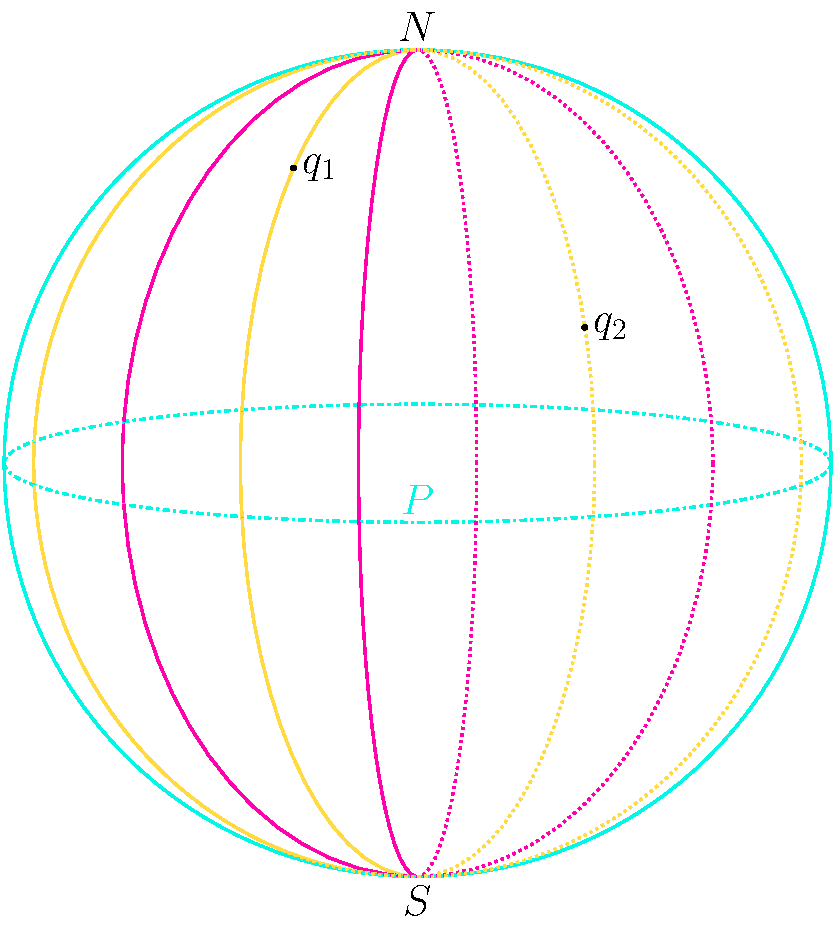
\includegraphics[scale=0.42]{Immagini/sphere-focal-points/sphere-focal-points.pdf}
\caption[]{The yellow solid curve is the shortest path from \(P\) and \(q_1\), but cannot be length minimizing after the north pole (focal point of \(P\) along that curve). Indeed the minimizing path from \(P\) to \(q_2\) is the other yellow dotted curve.}
\label{fig:sphere-focal-points}
\end{wrapfigure}

We have seen that they represent \emph{almost} meeting points of congruences of geodesics of the same causal character; now, if we were to study geodesics in a Riemannian manifold, the relation between the presence of focal points and the failure of minimizing the distance between \(2\) points would be quite clear, not only geometrically but also by the analytical study of the length functional.

In the case of (strictly) timelike geodesics, there exists a good analog of Riemannian distance: the proper elapsed time; in a globally hyperbolic spacetime there will always exists a curve that maximizes the elapsed proper time - so a path that represents the slowest trip - between \(2\) points, and again, past a focal point a timelike geodesic cannot be \(\tau-\)maximizing anymore.

However, for null geodesics the proper elapsed time is always zero, so these geodesics will always be \(\tau\)-minimizing; in parallel, we have already said that the length functional is not smooth on this set of curves, and that was the reason for which we needed to study \(E\) instead of \(L\). But is there any analog of the length-minimizing property, whose loss corresponds to the presence of focal points? Well, the answer is yes: Witten calls it \emph{promptness}~\cite{witten2020light}.

\begin{definition}
	A path \(\gamma\) from \(P\) to \(q\) is \emph{prompt} if there is no causal path \(\gamma'\) from \(p\) to any point in the past of \(q\), \(q'\in J^-(q)\).
\end{definition}

The idea is that a prompt path is the ``fastest'' possible way for an event to reach some place, in the sense that no information about that event can possibly arrive earlier.

Prompt causal paths bear some interesting properties:
\begin{itemize}
	\item[\ding{99}] A prompt path between \(p\) and \(q\) can only exist if \(q\in\partial J^+(p)\), so if it is just barely possible to reach \(q\) from \(p\) through a causal path.
	\item[\ding{99}] A path is prompt if and only if it is an \emph{achronal} null geodesic, orthogonal to \(P\).
	\item[\ding{99}] If strong causality holds every null geodesics has an initial segment which is prompt; conversely, the prompt part of a null geodesic has to be an initial segment, because continuing further a null geodesic which is not prompt anymore, cannot make it prompt again.
	\item[\ding{99}] To be prompt, a null geodesic must not contain any focal point.
\end{itemize}

It is interesting to see how in section \(8\) of the same reference Witten tries to emancipate the analysis of focal points from Raychaudhuri's equation, and arrives to the formulation of a functional \(\tilde{J}(x^A)\) to be minimized.

He points out the parallel between this procedure and a sort of Shr\"odinger formulation of the problem by seeking out an hamiltonian such that:
\[
	\tilde{J}(x^A) = \langle \psi \vert H \vert \psi \rangle.	
\]
The only problem with his formulation is that, although realizing the presence of some surface terms in \(\tilde{J}(x^A)\), he doesn't clearly write them down, but leave them hidden in some unknown function (that he calls \(f_2(x^A(0))\)). We will see instead that it is crucial for us to express that term as contraction of the mean normal curvature with the tangent field.
